\documentclass[times,final]{elsarticle}
%%
%\documentclass[times,twocolumn,final,longtitle]{elsarticle}
%%
%% Compress citation scheme
\biboptions{numbers,sort&compress}

%% Stylefile to load JCOMP template
\usepackage{jcomp}
\usepackage{framed,multirow}

%% The amssymb package provides various useful mathematical symbols
\usepackage{mathrsfs}
\usepackage[fleqn]{amsmath}
\usepackage{amssymb}
\usepackage{latexsym}

% Following three lines are needed for this document.
% If you are not loading colors or url, then these are
% not required.
\usepackage{url}
\usepackage{xcolor}
\definecolor{newcolor}{rgb}{.8,.349,.1}

%% Define a new 'leo' style for the package that will use a smaller font.
\makeatletter
\def\url@leostyle{%
  \@ifundefined{selectfont}{\def\UrlFont{\sf}}{\def\UrlFont{\small\ttfamily}}}
\makeatother

%% Now actually use the newly defined style.
\urlstyle{leo}

%%insert figures
\usepackage{caption}
\usepackage{graphicx}
\usepackage{epstopdf}
%\usepackage{graphicx,times}
\usepackage{subfigure}
\usepackage{natbib}
\usepackage{geometry}
%\geometry{left=2cm,right=2cm,top=2cm,bottom=2cm}
\graphicspath{{pictures/}}
\journal{Journal of Computational Physics}
\begin{document}
\verso{Given-name Surname \textit{etal}}

\begin{frontmatter}

\title{A coupled level set and volume of fluid method for sharp interface simulation}%

\author[1]{Linfan \snm{Zhang}\corref{cor1}}
\cortext[cor1]{Corresponding author:
  Tel.: +0-000-000-0000;
  fax: +0-000-000-0000;}
\author[1]{Weimin \snm{Ma}\fnref{fn1}}
%\fntext[fn1]{This is author footnote for second author.}
%\author[2]{Arthur \snm{Morgan}}
%% Third author's email
\ead{zlf0030@163.com}
%\author[2]{Edward \snm{Conway}}

\address[1]{Affiliation 1, Address, City and Postal Code, China}
\address[2]{Affiliation 2, Address, City and Postal Code, Country}

\received{1 Jan 2019}
\finalform{10 Jan 2019}
\accepted{13 Jan 2019}
\availableonline{15 Jan 2019}
%\communicated{S. Sarkar}


\begin{abstract}
 This paper presents a coupled level-set and volume-of-fluid method for unstructured meshes. This method designed for simulating incompressible two phase flows combines both the advantages of LS method and VOF method. The method is called CLSAdvector, and is implemented into OpenFOAM$^{\textregistered}$ as open source. Volume of fluid (VOF) idea is conservative because it can calculate the volume of one of the fluids transported across the mesh faces in a time step. In contrast to VOF, the LS method provides a sharp interface and a smooth transition in the physical properties across the interface. The novelty of the CLSAdvector concept combines the ideas of VOF and LS method. First, an algorithm is designed for calculating the position of interface inside cells where the void fraction and the direction of interface are given. Second, the level set function is limited in a narrow band that contains the interface, which improves the efficiency of the algorithm. The feasibility and accuracy of the current method are validated by several cases including Zalesak's problem, 2D vortex, dam break, and jet break-up.
\end{abstract}
\begin{keyword}
interfacial flows\sep CLSAdvection \sep CFD \sep OpenFOAM$^{\textregistered}$
%\KWD Keyword1\sep Keyword2\sep Keyword3
\end{keyword}

\end{frontmatter}

\section{Introduction}
%The main method of interface capturing. VOF,front tracking, level set, coupled VOF and level set.
%1. The application of multi-phase flow in engineering and physics especially in nuclear safety.
%2. The importance of interface capture method in the simulation of multi-phase flow
%3. The variety of interface capture methods and the latest research on them.
% Interface capture and multiphase flow
Incompressible two phase flow with large density ratio at the free surface can be found in many natural phenomenon and industrial processes such as power plant, internal combustion, chemical reactor. Especially during nuclear reactor severe accidents, the molten corium from the fuel core region or the reactor pressure vessel (RPV) may fall into water pool. Then fuel coolant interaction (FCI) will happen and can lead to steam explosion which can cause severe damage to the containment of the nuclear reactor. Severity of steam explosion can be decided by the limited breakup of the molten pour stream flowing through the water prior to stream explosion\cite{Ginsberg1986Liquid}. In order to study the effect of melt physical properties on the jet breakup length and the characterization of droplet size distribution in the premixing region, it is crucial to track molten and water interface motion precisely.

%Main interface capture methods
Computing interface motion plays an important role in numerical multi-phase flows research. There are several methods developed for interface tracking or capturing in multi-phase Computational Fluid Dynamics (CFD) and different methods have their own characteristics. In general, the interface tracking method and interface capturing method are the two main classes of methods that are used to locate the interface. Both the classes are validated against a Taylor bubble benchmark problem by Marshall \textit{et al.}\cite{marschall2014validation}.

Interface tracking methods includes the arbitrary Lagrangian-Eulerian (ALE) method and the marker and cell (MAC) method. A typical ALE method is front tracking method \cite{Unverdi1992A,TRYGGVASON2001708}, which is based on an adaptive mesh that deforms with the interface that is advected in a Lagrangian fashion by the velocity interpolated from the CFD velocity field. MAC method use a series of points inside a fixed-grid region to represent the interface. The points are moved in Lagrangian fashion in the velocity field solved from Navier-Stokes equations. Interface tracking method can precisely describe the motion of interface but can not strictly conserve mass and the algorithm can be very sophisticated and time-consuming when the interface is deeply twisted. And this method is still under development and improvement. Mari{\'c} \textit{et al.} implemented a compromising hybrid Level Set/Front tracking Method for unstructured grids within OpenFOAM framework \citep{MARIC201520}.

The interface capturing methods as another approach to simulate free surface and interfacial flows mostly include the volume of fluid(VOF) method\cite{hirt1981volume,rudman1997volume} and the level set(LS) method\cite{Sussman1994A,chang1996level}, which both adopt a scalar function to capture the interface in fixed Eulerian grids. Currently the interfacial flow solvers take variants VOF methods as the interface advection step in most CFD codes, which include current versions of ANSYS Fluent$^{\textregistered}$, STAR-CCM++$^{\textregistered}$,OpenFOAM$^{\textregistered}$ and so on. The VOF method defines void fraction $\alpha$ as the fraction of volume occupied by the liquid in each cell. The void fraction $\alpha$ bounded between 0 and 1 at the cells fully occupied by one of phases, changes discontinuously across the interface. The most crucial step of the method is to solve the advection equation of $\alpha$. But due to the discontinuous nature of $\alpha$, large numerical diffusion in the convection scheme causes non-physical smearing of the interface. In order to describe the interface precisely, most VOF methods are separated into two categories, geometric VOF \cite{diot2016interface,hirt1981volume,Gueyffier1999Volume,NohAndWoodward1976,RIDER1998112,Youngs1982,roenby2016computational,puckett1997high} and algebraic VOF \cite{rudman1997volume,Muzaferijia1998,Ubbink1997,weller2008new,rusche2003computational,deshpande2012evaluating}. Geometric VOF methods define or reconstruct the interface location within a cell using the function value $\alpha$, while algebraic VOF methods use high solution schemes and compressive to reduce the numerical diffusion without defining exactly the location of interface.
%%\subsubsection{Geometrical VOF}

Generally, the interface described by the geometrical methods is more accurate and less smeared than the algebraic methods. Because in most geometrical methods, the interface segment is reconstructed within a cell volume by piecewise lines. During the past decades, scientists proposed variants geometrical methods, which include donor-acceptor\cite{hirt1981volume}, SLIC(simple line interface calculation)\cite{NohAndWoodward1976} and PLIC(piecewise linear interface calculation)\cite{Youngs1982}. The PLIC method is a second-order algorithm and the reconstructed interface is much shaper than other geometrical methods.The article\cite{rudman1997volume} summaries the three geometrical methods and compares them with FCT(flux-corrected transport)-VOF method proposed in the article. The conclusion is that Youngs' method\cite{Youngs1982} may be more accurate but more complicated to apply in three dimensions and unstructured meshes than FCT-VOF methods. To be applied for three dimensions, the piecewise-linear interface calculation method is proposed in \cite{Gueyffier1999Volume}. And the interface reconstruction method is realized in \cite{diot2016interface} for three dimensional arbitrary convex cells. One of the geometrical algorithms called isoAdvector is proposed in \cite{roenby2016computational} and implemented into OpenFOAM$^{\textregistered}$ as the incompressible two-phase flow solver, isoAdvector. This method uses the concept of isovalue contours to locate the interface in cells. For full details, the source code is provided with this website\cite{isoAdvector}.
%%\subsubsection{Algebraic VOF}

Among algebraic methods, using standard upwind scheme to transport the VOF field is the easiest one to apply. Most algebraic methods use the compressive algorithms to discretize the convective term in the VOF advection equation for preserving the interface sharpness. The interface typically spreads over a few cells and diffuses lowly but unboundedly under certain conditions\cite{Ubbink1997}. The interface smearing can be minimized and bounded by adding a compressive term or counter gradient term to the VOF advection equation\cite{weller2008new}. Some solvers like interFoam and multiphaseInterFoam in OpenFOAM$^{\textregistered}$ use the algebraic methods, also called Multidimensional Universal Limiter with Explicit Solution (MULES) algorithm, which is highly adaptive to three dimensions and unstructured grids. The performance of the two-phase flow solver - interFoam is evaluated in \cite{deshpande2012evaluating} and the basic principle of MULES algorithm can also be found.

%%\subsection{Level set methods}
%%Level set function.
 Level set method was first proposed by Osher and Sethian \cite{osher1988fronts}, and then it was coupled to the equations for two-phase incompressible flow by Sussman \textit{et al.}\cite{Sussman1994A}. LS method was proved to be a powerful algorithm to handle complex topological changes such as merging, twisting and pinching by following research \cite{Sussman1995A,chang1996level,sussman1998improved}. And exhaustive explanation and general applications of LS method can be found in Osher and Fedkiw's book\cite{osher2006level} and Sethian's book\cite{sethian1999level}. In stead of using bounded volume fraction, the idea of LS method is to represent the interface with the zero value iso-face of a level set function $\phi$. The value of $\phi$ is positive in one phase and negative in the other \cite{chopp1991computing}. One advantage of LS method is that the interface is advected implicitly by solving the advection equation of $\phi$, which solved algebraically with high order discretization schemes like WENO (weighted essentially non-oscillatory) scheme \cite{liu2017coupled,son2002coupled,martin2018implementation}.
%%Reinitialization function.
Due to the Lipschitz-continuous nature of the level set function, which is usually takes the form of the signed distance to the interface, the derivatives of $\phi$ are easy to calculate as well as the normal and curvature of the interface \cite{ge2018efficient}. The signed distance function prevents gradients of $\phi$ from being steep and flat as that can cause numerical instabilities and loss inaccuracy.  As $\phi$ is advected by solving the transport equation, the interface's shape is changed and the level set function loses the characteristic of the signed distance function that can be restored by reinitialization equation\cite{Sussman1994A,Johansson422383}. However, mass loss/gain always occurs along with the simulation of incompressible flows, because LS function can not provide volume information as VOF does. Furthermore, numerical errors arise from solving the LS advection equation and/or the reinitialization equation. Especially in areas of high curvature or other unsolved regions, the discretization of advection equation can cause inevitable and significant numerical dissipation\cite{losasso2006spatially}. Many attempts have been made to improve the mass conservation of the level set method and reduce numerical dissipation from advection equation and reinitialization process. This article \cite{luo2015mass} summarized several glories of improvement strategies.

A lot of studies were devoted to improve level set method. Some applied high solution schemes like fifth-order WENO scheme\cite{nourgaliev2005improving,salih2009some}, discontinuous Galerkin method \cite{reed1973triangular,rasetarinera2001efficient,remacle2007efficient} and semi-Lagrangian approach\cite{enright2005fast,strain1999semi,xiu2001semi}. Some articles studied velocity extensions method to maintain the signed distance function\cite{adalsteinsson1999fast,chopp2009another,ovsyannikov2012new,sabelnikov2014modified}. Moreover, using hyperbolic tangent function to supersede the signed distance function as the level set function was firstly proposed by Olsson \textit{et al.}\cite{OLSSON2005225,OLSSON2007785}. A series of work based on the method has been done\cite{chiodi2017reformulation,chiu2011conservative,sato2012conservative,sheu2009development,sheu2011development,NONOMURA201495,owkes2013discontinuous,xiao2005simple,walker2010conservative,desjardins2008accurate}. But small pieces of fluid are found breaking off from the interface and moving with erroneous velocity field\cite{luo2015mass}. Besides, Kohno \textit{et al.} \cite{KOHNO20131547} proposed a novel numerical method for solving the advection equation for a level set function by using hierarchical-gradient truncation and remapping (H-GTaR) of the original PDE. In addition, spatially adaptive level set methods were developed to improve the accuracy of the interface location. These methods include the adaptive level set approach\cite{sussman1999adaptive}, the octree based methods \cite{losasso2006spatially,fuster2009simulation}, the structured adaptive mesh refinement\cite{nourgaliev2005improving}, the refined level set grid (RLSG) method \cite{herrmann2008balanced}, the spectrally refined interface approach \cite{desjardins2009spectrally} and the adaptive level set method\cite{kim2011accurate}. These articles\cite{nguyen2001boundary,Gihun2005,GIBOU2007536,tanguy2005application} combined LS method with Ghost FLuid Method \cite{fedkiw1999non} and the boundary conditional capturing technology\cite{liu2000boundary}. On the other hand, Some studies are aimed for improving the accuracy and efficiency of the reinitialization process\cite{sussman1998improved,sussman1999efficient,RUSSO200051,HARTMANN20086821}. There are several ways to restore the signed distance function, including PDE (partial differential equation) method \cite{peng1999pde,chang1996level,MCCASLIN2014408} and FMM (fast marching method) \cite{adalsteinsson1995fast,sethian1996fast,sethian2001evolution,salac2011augmented,desjardins2009spectrally,desjardins2008accurate}. Besides, more sophisticated methods for reinitialization have been proposed, including geometric mass-preserving redistancing scheme \cite{ausas2011geometric} and the volume-reinitialization scheme\cite{salih2013mass}.Hysing and Turek discuss and compare these reinitialization methods in \cite{hysing2005eikonal}.

%(1) High solution schemes like fifth-order WENO scheme can improve the accuracy and reduce mass losses\cite{nourgaliev2005improving,salih2009some}. Discontinuous Galerkin method was created by Reed and Hill\cite{reed1973triangular}. These articles\cite{rasetarinera2001efficient,remacle2007efficient} applied this method in the discretization of the level set equation because of its high-order accurate compact scheme. In addition, the semi-Lagrangian approach has been applied to the discretization of the level set function by first-order schem\cite{enright2005fast,strain1999semi} and high-order scheme\cite{xiu2001semi}.

%(2) Velocity extensions are used to map the velocity of interface into the rest of computational domain\cite{adalsteinsson1999fast}, which is based on the fact that the gradient of the level set function grows rapidly in shearing velocity fields\cite{chopp2009another}. Extensive velocity method can maintain the signed distance function by introducing the source term into the advection equation. But first-order approximation still causes numerical artifacts which leads to higher-order schemes applied in the method\cite{ovsyannikov2012new,sabelnikov2014modified}.

%(3) Hyperbolic tangent function is used by THINC (tangent of hyperbola for interface capturing) scheme to supersede the signed distance function as the level set function, which is firstly proposed by Olsson \textit{et al.}\cite{OLSSON2005225,OLSSON2007785}.A lot of work based on the method has been done\cite{chiodi2017reformulation,sato2012conservative,sheu2009development,sheu2011development,NONOMURA201495,owkes2013discontinuous,xiao2005simple,walker2010conservative,desjardins2008accurate}. But small pieces of fluid are found breaking off from the interface and moving with erroneous velocity field\cite{luo2015mass}. Besides, Kohno \textit{et al.} \cite{KOHNO20131547} proposed a novel numerical method for solving the advection equation for a level set function by using hierarchical-gradient truncation and remapping (H-GTaR) of the original PDE.

  %*Chang \textit{et al.}\cite{chang1996level} proposed a re-initialization procedure involving a perturbed Hamilton-Jacobi equation to a steady state. *McCaslin and Desjardins \cite{MCCASLIN2014408} further improved the reinitialization equation to account for significant amount of spatial variability in level set transport. Another reinitialization method FMM proposed to reduce computational cost was extended to get higher-order accuracy\cite{desjardins2009spectrally,sethian1999level,desjardins2008accurate}. Other methods for reinitialization have been proposed, including geometric mass-preserving redistancing scheme \cite{ausas2011geometric} and the volume-reinitialization scheme\cite{salih2013mass}.

To take advantages of both LS and VOF methods, Sussman \textit{et al.}\cite{SUSSMAN2000301,SUSSMAN2003110} proposed a coupled level set and volume of fluid (CLSVOF) method. These studies applied CLSVOF method and its variants\cite{wang2012new,wang2010sharp,lv2010novel,menard2007coupling,yang2006adaptive,son2003efficient}.
Some improved CLSVOF methods, like VOSET method\cite{sun2010coupled},the conservation correction equation method\cite{kees2011conservative}, and the level set volume constraint method\cite{wang2012hybrid} were developed. Cao \textit{et al.}\cite{cao2018coupled} applied VOSET method based on multi-dimensional advection for unstructured triangular meshes. Pijl \textit{et al.} \cite{van2008computing,van2005mass} proposed a mass-conserving method, which does not need to construct the complicated interface. Besides, these articles\cite{le20133d,trontin2012subgrid,hieber2005lagrangian,enright2002hybrid} applied the hybrid Lagrangian-Eulerian method to rebuild the level set function.

%(6)Spatially adaptive level set methods were developed to improve the accuracy of the interface location. These methods include the adaptive level set approach\cite{sussman1999adaptive}, the octree based methods \cite{losasso2006spatially,fuster2009simulation}, the structured adaptive mesh refinement\cite{nourgaliev2005improving}, the refined level set grid (RLSG) method \cite{herrmann2008balanced}, the spectrally refined interface approach \cite{desjardins2009spectrally} and the adaptive level set method\cite{kim2011accurate}.

In this paper, we introduce the CLSAdvection algorithm which is a mass conservative level set method coupled with volume of fluid method. The purpose of developing this algorithm is to combine the continuous nature of level set function $\phi$ and the mass conservative property of void fraction $\alpha$. CLSAdvector algorithm significantly reduces the smearing of the interface and avoids the mass loss caused by numerical diffusion. This algorithm is developed into a multi-phase solver implemented in the OpenFOAM$^{\textregistered}$ CFD software.

In the reminder of this section, we review the interface problem and all kinds of previous studies on the interface tracking/captring methods. In section 2, we introduce the concept of CLSAdvector algorithm and give an overview of the steps involved in the numerical procedure. In section 3, the corresponding numerical implementations are presented in detail. This is followed by section 4, in which four benchmark case are tested for validation. Finally, some conclusions are drawn in section 5.

\section{The CLSAdvection concept}
The idea of CLSAdvector was inspired by Roenby \textit{et al.} who proposed isoAdvector concept\cite{isoAdvector}, which is a geometric VOF method. In the isoAdvector method, void fraction $\alpha$ is interpolated into the vertexes of the grids. Generally, it is customary to visualize the interface by showing the 0.5-isosurface based on the void fraction $\alpha$ with the post-processing procedure, like ParaView$^{\textregistered}$. However, it is not precise to use 0.5-isosurface as interface because it can hardly cut the cell into two subcells of the volumetric proportions dictated by the volume fraction $\alpha$. So the most important step of isoAdvector is to find the exact value of $\alpha$ that can cut the surface cells into two subcells with right void proportions. This method is quite novel and it is applied to unstructured meshes and implemented as an incompressible two-phase flow VOF solver in OpenFOAM$^{\textregistered}$. However, isoAdvector still has the same faults as other geometric VOF methods, in which the curvature and normal direction of interface are influenced by the discontinuous property of $\alpha$. Different from the isoAdvector method, CLSAdvector uses the projection distance D of $\vec{x}_j$ (the vector from cell center to \textit{i}-th vertex) on interface normal direction $\vec{n}$ to reconstruct the interface that meets void fraction $\alpha$. For the sake of clarity, only ideas about CLSAdvector are focused in this section, and the numerical detailed description of the implementations can be found in section 3. The reader is referred to the source code provided at this website\cite{CLSAdvector}.
\subsection{Governing equations for incompressible two phase flow}
%Navier-Stokes Momentum equation
The incompressible Navier-Stokes equations for two immiscible phases(A and B) read
\begin{equation}\label{1}
\frac{\partial \mathbf{u}}{\partial t}
+ \mathbf{u}\cdot\nabla\mathbf{u}
=
-\frac{1}{\rho}\nabla{p}
+\frac{1}{\rho}\nabla\cdot(2\mu{D})
+\mathbf{f_\Gamma}
+\mathbf{g}
\end{equation}
%Navier-Stokes Conservative equation
\begin{equation}\label{2}
\nabla\cdot\mathbf{u}=0
\end{equation}
where $\mathbf{u}$ is the velocity, $\rho$ is the density, \textit{p} is the pressure, $\mathbf{g}$ is the gravitational acceleration and $\mu$ is the dynamic viscosity. The material properties are constant for each phase and discontinuous at the interface. To avoid numerical instability \cite{son2002coupled}, it is needed to make fluids properties in a continuous form as follows
\begin{equation}\label{16}
\rho=\rho_A + (\rho_B-\rho_A)H(\phi),
\end{equation}
and
\begin{equation}\label{17}
\mu=\mu_A + (\mu_A-\mu_B)H(\phi).
\end{equation}
In equation \ref{1}, D is defined as the rate of deformation tensor,
\begin{equation}\label{3}
D=\frac{\nabla\mathbf{u}+{\nabla\mathbf{u}}^T}{2}.
\end{equation}
$\mathbf{f_\Gamma}$ is the surface tension force, which is transformed to be a volume force scattering within the interface region by CSF (continuum surface force) model\cite{brackbill1992continuum} as follows
\begin{equation}\label{4}
\mathbf{f_\Gamma}
=
\frac{\sigma\kappa\nabla{H_\varepsilon(\phi)}}{\rho_\varepsilon(\phi)}.
\end{equation}
At the interface $\Gamma$, separating the two fluids, there is the normal continuity condition for velocity
\begin{equation}\label{5}
u_{A,\perp}-u_{B,\perp}
=
\mathbf{u}_A\cdot\mathbf{n}
-
\mathbf{u}_B\cdot\mathbf{n}
\equiv
0,
\end{equation}
the tangential continuity condition for velocity
\begin{equation}\label{6}
u_{A,\parallel}-u_{B,\parallel}
\equiv
0,
\end{equation}
and the jump condition for surface stress
\begin{equation}\label{7}
  [\mathbf{n}\cdot(-p\mathbf{I}+2\mu{D})\cdot\mathbf{n}]=\sigma\kappa,
\end{equation}
where $\mathbf{I}$ is the identity matrix, $\sigma$ is the surface tension and $\kappa$ is the interface curvature. According to the article\cite{van2008computing}, if viscosity is continuous across the interface, the coupled jump condition of pressure and velocity gradient(\ref{7}) can be decoupled. Then we can get
\begin{equation}\label{14}
[\nabla\mathbf{u}]_\Gamma = 0,
\end{equation}
and
\begin{equation}\label{15}
[p]_\Gamma=\sigma\kappa.
\end{equation}
The curvature $\kappa$ is calculated from
\begin{equation}\label{9}
\kappa=-\nabla\cdot\mathbf{n}=-\nabla\cdot\frac{\nabla\phi}{\left|\nabla\phi\right|},
\end{equation}
where $\mathbf{n}$ is the unit normal vector.
The jump conditions for pressure and materials are smeared out over the interface region of a thickness $\eta=2\varepsilon$. A smoothed Heaviside function is applied to make the jump conditions smeared and continuous as follows
\begin{equation}\label{8}
H_\varepsilon(\phi)=
\left\{
\begin{array}{ll}
0, & {\phi<-\varepsilon} \\
\frac{1}{2}[1+\frac{\phi}{\varepsilon}+\frac{1}{\pi}\sin{(\pi\frac{\phi}{\varepsilon})}],& {\left|\phi\right|\le{\varepsilon}}.\\
1, & {\phi>\varepsilon}
\end{array}\right.
\end{equation}

\subsection{Interface reconstruction}
The kernel of CLSAdvector algorithm is to reconstruct interfaces in surface cells with normal direction $\mathbf{n}$ calculated from $\phi$ and void fraction $\alpha$. First of all, it is necessary to define the volume fraction $\alpha$ of fluid phase A in cell $i$ at time $t$,
\begin{equation}\label{18}
\alpha_i(t)\equiv\frac{1}{V_i}\int_{\mathscr{C}_i}\Pi(\mathbf{x},t)dV
\end{equation}
where $\Pi$ is a characteristic function,
\begin{equation}\label{19}
\Pi(\mathbf{x},t)\equiv\left\{
\begin{array}{lr}
1,&\mathbf{x}\in Phase A \\
0,&\mathbf{x}\in Phase B.
\end{array}\right.
\end{equation}
Although the interface may be actually curved inside a surface cell, it is approximately regarded as a plane inside the cell. In order to locate the position of interface with the two important variables $\mathbf{n}$ and $\phi$ in a polyhedral cell, in CLSAdvection method, iso-value surfaces which can cut the cells into the correct ratio are calculated. In order to find this iso-value for a given surface cell, an efficient method is proposed and the details can be seen at section 3. We have to admit that the iso-value faces are not continuous because they are designed to meet the mass conservative condition as we can see in figure \ref{fig:noncontinuous}. Therefore, the reconstructed interfaces are only used to calculate the void fraction field of the next time step by simulating the motion of the interface, while the normal direction $\mathbf{n}$ is provided by solving the advection of level set function.

\begin{figure}[htbp]
\centering
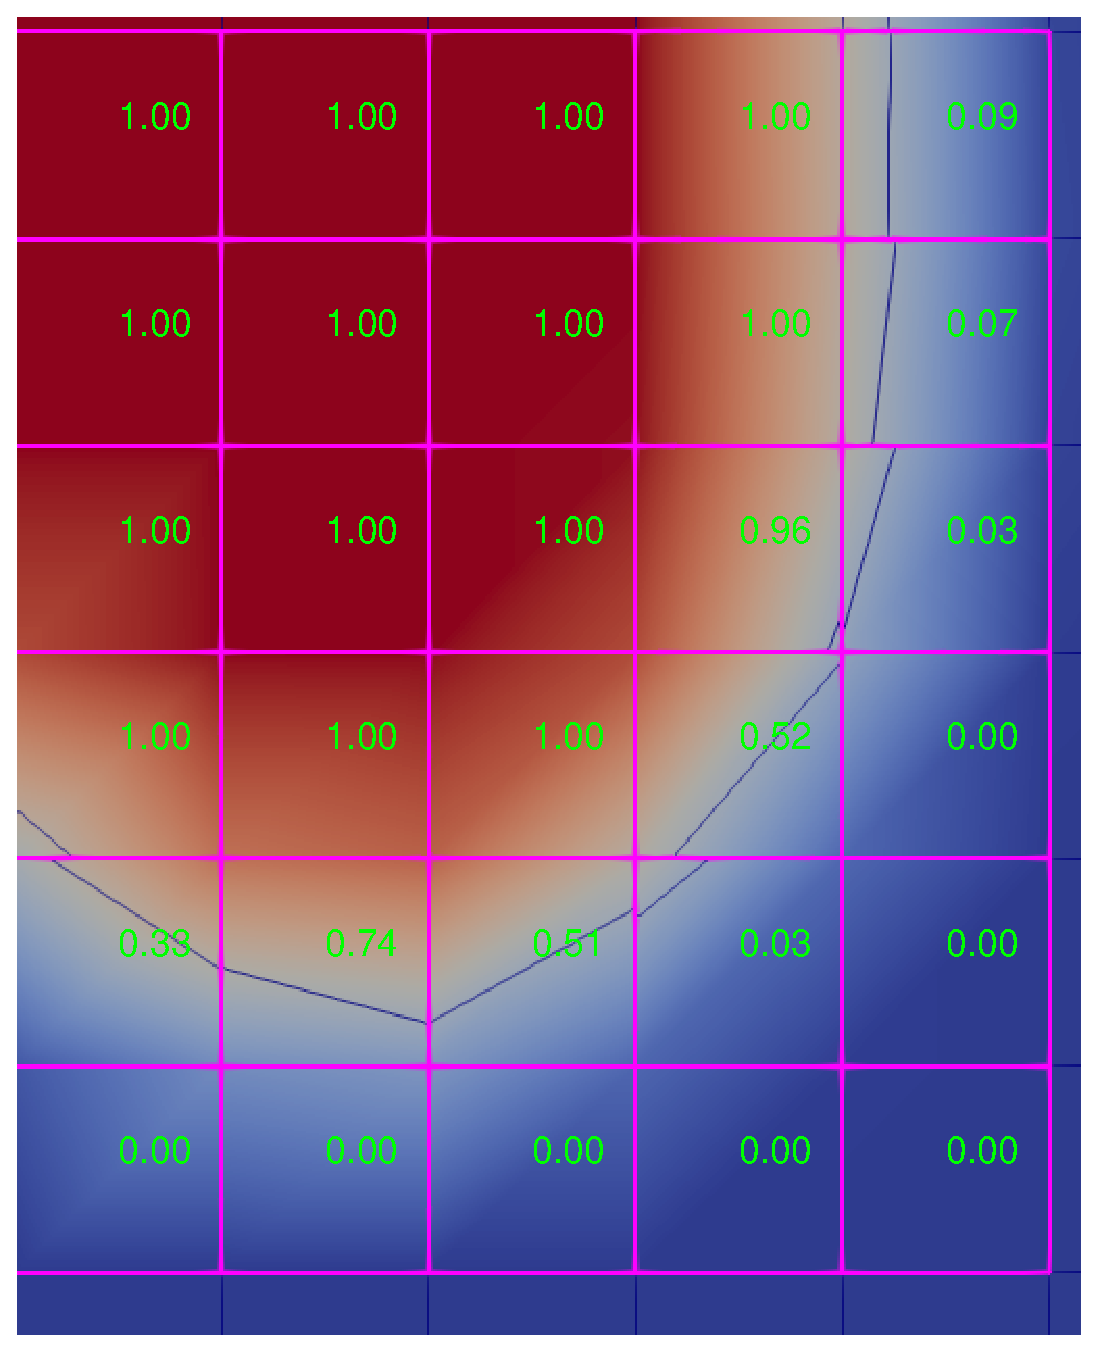
\includegraphics[width=0.4\textwidth]{noncontinuous.eps}
\caption{Noncontinuous reconstructed interfaces}
\label{fig:noncontinuous}
\end{figure}

\subsection{Interface motion}
The following equation for the volume of fluid is solved to keep the free surface conservative,
\begin{equation}\label{13}
\frac{\partial\alpha}{\partial{t}}+(\mathbf{u}\cdot\nabla)\alpha=0.
\end{equation}
As the system of all governing equations is solved in sequence within a time step, only the information about velocity field $U$, void fraction $\alpha$ and level set function $\phi$ at time $t$ is available. The void fraction field of the next time step is calculated by the following function,
\begin{equation}\label{22}
\alpha_i(t+\Delta{t})=\alpha_i(t) - \frac{1}{V_i}\sum_{j\in\mathscr{B}_i}\sigma_{ij}\int_t^{t+\Delta{t}}\int_{\mathscr{F}_i}{\Pi(\mathbf{x},\tau)\mathbf{u}(\mathbf{x},\tau)}{d\mathbf{S}d\tau},
\end{equation}
where $\sigma_ij\in{+1,-1}$, such that $\sigma_{ij}{d\mathbf{S}}$ on each cell face points from cell $i$ to cell $j$. The information between the interval $[t,t+\Delta{t}]$ is unknown. Hence it is simply estimated that the velocity field is regarded as constant during the time step. Besides, the velocity $\mathbf{u}(\mathbf{x},t)$ on the cell face is dotted with differential face normal vector, $d\mathbf{S}$, which is difficult to be integrated because of the unknown distribution of velocity on the cell face. This term can be approximated as average velocity, $u_{ij}(t)$, multiplied with differential face as follows:
\begin{equation}\label{24}
  \mathbf{u}(\mathbf{x},t)d\mathbf{S}\approx u_{ij}(t)dS =\frac{F_{ij}(t)}{S_{ij}}dS,
\end{equation}
where volumetric face flux, $F_{ij}$, is defined to estimate the average velocity on the cell faces,
\begin{equation}\label{23}
  F_{ij}(t)\equiv\int_{\mathscr{F}_{ij}}\mathbf{u}(\mathbf{x},t)d\mathbf{S}.
\end{equation}
Substitute this into (\ref{22}) and we can have
\begin{equation}\label{24}
  \alpha_i(t+\Delta{t})=\alpha_i(t) - \frac{1}{V_i}\sum_{j\in\mathscr{B}_i}\sigma_{ij}\frac{F_{ij}(t)}{S_{ij}}\int_t^{t+\Delta{t}}\int_{\mathscr{F}_i}{\Pi(\mathbf{x},\tau)dSd\tau}.
\end{equation}
The remaining face integral means the area submerged in fluid A at time t, $\mathscr{A}_{ij}(t)$,
\begin{equation}\label{25}
  \mathscr{A}_{ij}(t)\equiv\int_{\mathscr{F}_i}{\Pi(\mathbf{x},t)}dS.
\end{equation}
The volume of fluid A across each cell face in time interval $[t,t+\Delta{t}]$ can be approximated with following equation,
\begin{equation}\label{26}
  \Delta{V}_{ij}(t,\Delta{t})\approx\frac{F_{ij}(t)}{S_{ij}}\int_t^{t+\Delta{t}}\mathscr{A}_{ij}(\tau)d\tau.
\end{equation}
As above equations show, in order to calculate the void fraction $\alpha_{i}(t+\Delta{t})$ at the next time step, it is necessary to calculate the area submerged by the reconstructed interface during $\Delta{t}$ and summarize the volume of fluid A, $\Delta{V}_i$ across each face of the cell. The algorithm of estimating the interface motion was proposed by Johan Roenby \textit{et al.} and can be found in \cite{roenby2016computational}.

\subsection{Level set function initialization}
At time $t$, the void fraction field $\alpha(t)$ is known. In volume of fluid method, the normal direction $\mathbf{n}$ is calculated by following equation,
\begin{equation}\label{27}
  \mathbf{n}=\frac{\nabla{\alpha}}{\left|\nabla{\alpha}\right|}.
\end{equation}
However, $\alpha$ field has discontinuous characteristic, $\alpha\in[0,1]$, which can lead to large numerical diffusion and non-physical smearing of the interface. Hence it is difficult to obtain high precision normal direction and curvature with VOF method especially for unstructured grid \cite{cao2018coupled}. To improve the interface capturing method, level set function $\phi$ with continuous characteristic at the interface is used in CLSAdvection method. The normal direction of interface is defined as follows,
\begin{equation}\label{20}
\mathbf{n}=\frac{\nabla\phi}{\left|\nabla\phi\right|}.
\end{equation}
The level set function field $\phi(t)$ at time $t$ can be obtained from the volume fraction field $\alpha(t)$ with following steps. First, the interface cells are found with the condition that $\alpha_i\in(0,1)$ and signed with flag $0$. Secondly, find its first layer around the interface cells and sign all the first layer cell with flag $1$. Do the same with second layer cells and sign them with flag $2$. Both the layers limit the thickness of the interface and ensure its precision. Thirdly, it is assumed that the continuous interface is the iso-surface at $\alpha=0.5$ and initialize the $\phi$ with following equation,
\begin{equation}\label{28}
\tilde{\phi}(t)=1.5\varepsilon(2*\alpha(t)-1).
\end{equation}
Apparently, the first initialized level set function $\tilde{\phi}$ is not the signed distance function. There are lots of methods to re-initialize the level set function, including partial differential equation method (PDE) and fast marching method (FMM). PDE method can be easily realized in unstructured grid for it is only need to solve the following re-initialization equation, which is also a hyperbolic equation,
\begin{equation}\label{11}
\frac{\partial\phi}{\partial\tau}+sgn(\tilde{\phi})(\left|\nabla\phi\right|-1)=0,
\end{equation}
in which $sgn(\phi)$ is a sign function as following,
\begin{equation}\label{12}
sgn(x)=\left\{
\begin{array}{lc}
1,& x>0\\
0,& x=0\\
-1.& x<0
\end{array}
\right.
\end{equation}
In order to solve equation (\ref{11}), Godunov's method for discretizing the hyperbolic term  $sgn(\tilde{\phi})\left|\nabla\phi\right|$, is recommended in \cite{osher2006level}. After solving the re-initialization equation, the signed distance field $\phi$ is obtained. Nonetheless, it still need correction to ensure the mass conservative characteristic. At last, our interface can be implicitly expressed with level set function, which is confined in a band containing the interface to save computing resource. All the detailed numerical algorithms can be found in section 3.

\subsection{Normal direction and curvature}
It is already known that level set method has the advantage of computing accurate interface normal direction but the disadvantage of keeping mass conservation. Hence, the signed distance level set function $\phi$ is used to calculate the normal direction at the next time step $t+\Delta{t}$ by solving the following hyperbolic convective equation,
\begin{equation}\label{10}
\frac{\partial\phi}{\partial{t}}+(\mathbf{u}\cdot\nabla)\phi=0.
\end{equation}
Equation (\ref{10}) is sometimes referred to as the \textit{level set equation}, which was firstly proposed by Osher and Sethian \cite{osher1988fronts}. After the equation is discretized with the finite volume method (FVM), it is essential to choose a suitable scheme to compute the fluxes of $\phi$ at all boundary faces of interface cells\cite{martin2018implementation} .Because the formation of large gradients during the interface motion can cause spurious oscillations near discontinuities at the interface and lose of the interface sharpness\cite{pringuey2012large}. Using an arbitrarily Weighted Essentially Non-Oscillatory (WENO) scheme proposed by Pringuey and Cant \cite{pringuey2012high} can handle complex interface. WENO schemes have the ability to preserve the required sharpness of the interface in front-propagating problems and to deal with large gradients with discontinuities. \cite{bilger2017evaluation} takes the advantage of WENO scheme to solve equation(\ref{10}) and realize the coupled level set and volume of fluid in OpenFOAM$^{\textregistered}$ with a hyperbolic tangent function $\psi$, which is similar to Heaviside function, $H$ in equation(\ref{8}). Martin and Shevchuk\cite{martin2018implementation} apply semi-implicit WENO schemes using OpenFOAM$^{\textregistered}$ and the source code is open source used in this article's work. Besides, a third-order Total Variation Diminishing (TVD) Runge-Kutta(RK) scheme for temporal discretization is used for the advection steps\cite{pringuey2014robust}.

%\subsection{Dentisy and viscosity}
\subsection{Algorithm overview}
The numerical algorithm combines the method of volume of liquid  and level set. The solver start off with the initialization of velocity, pressure and $\alpha$ fields. Before the time loop, the LS variable, $\phi$, generate from the $\alpha$ field and create other variables like $\delta$ and $H$. Then PIMPLE loop starts from the interface reconstruction with $\alpha$ and $\vec{n}$. The figure (\ref{fig:AlgorithmProcess}) shows the specific flow chart.
\begin{figure}[htbp]
\centering
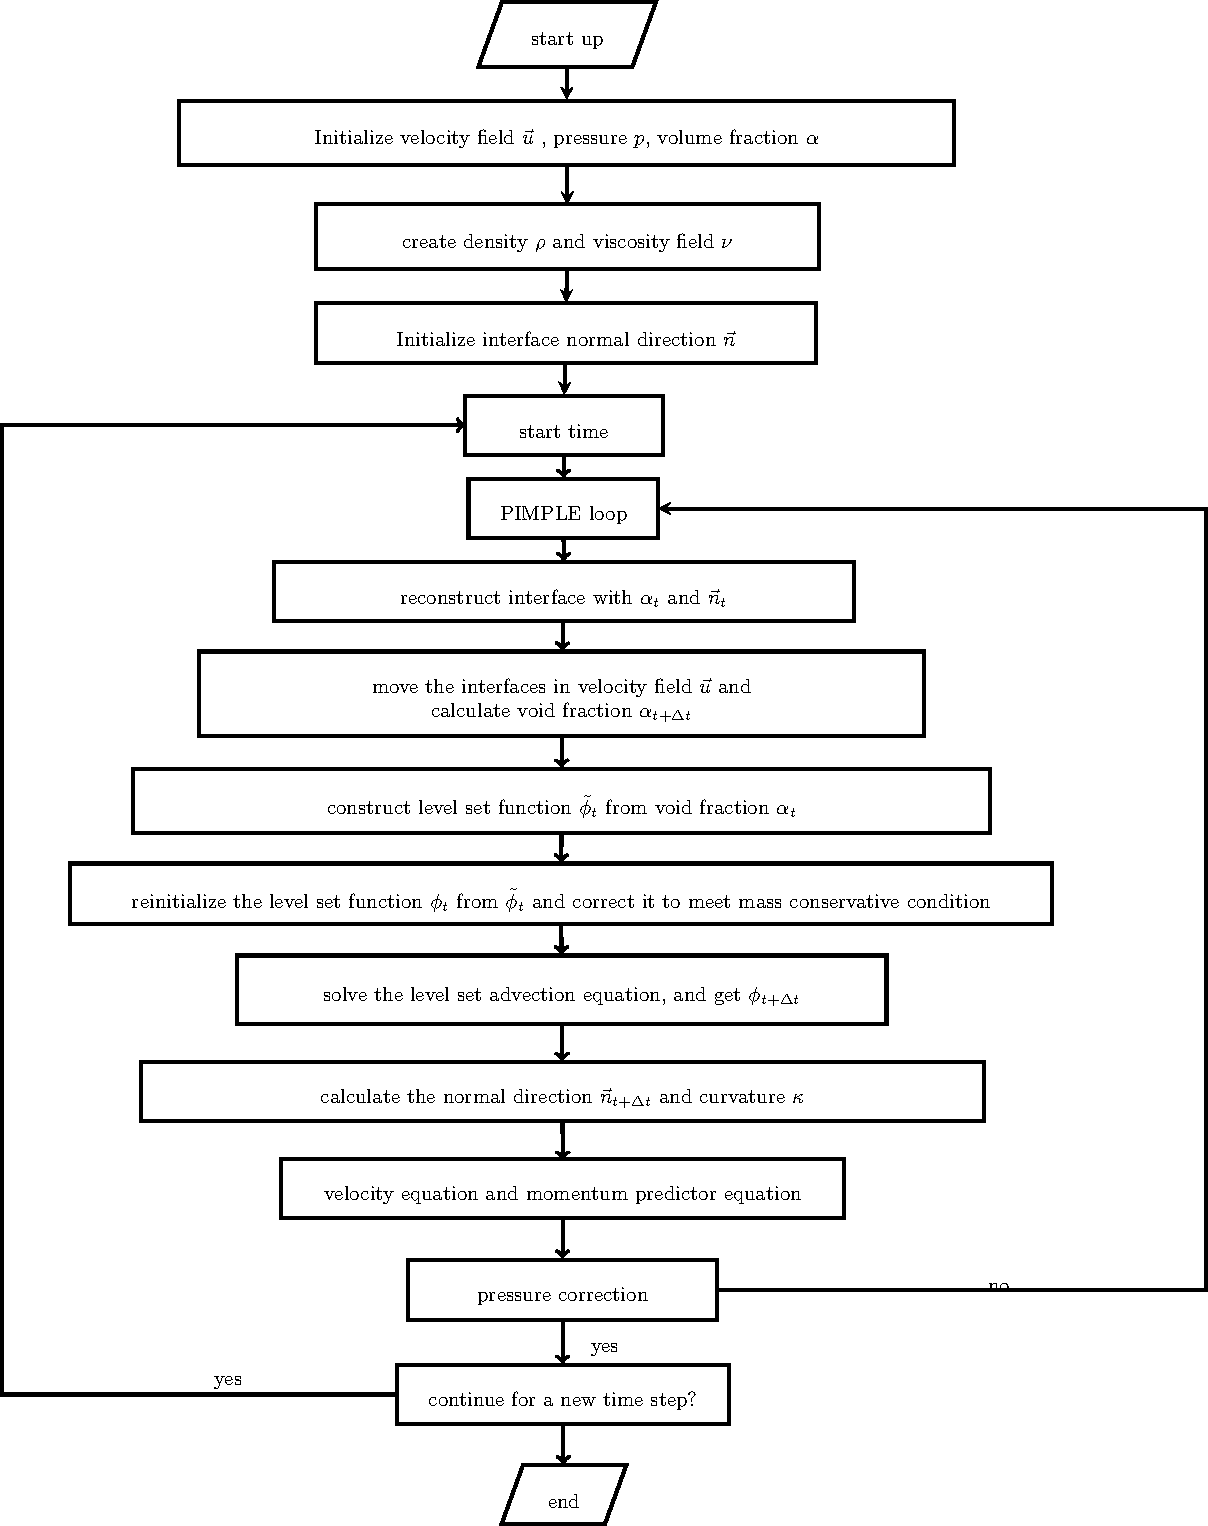
\includegraphics[width=1\textwidth]{Diagram.pdf}
\caption{Algorithm for the CLSAdvection solver.}
\label{fig:AlgorithmProcess}
\end{figure}
\section{Numerical implementations}
\subsection{Cutting the cell with $\alpha$ and $\phi$}
In this case, the normal direction $\mathbf{n}$ of certain cell is given by level set function $\phi$ and the void fraction $\alpha$ is given by volume of fluid function. This section means to explain the algorithm of finding such a plane with normal direction $\mathbf{n}$ that can cut the cell into the right void fraction $\alpha$. The locations of cell center point $\mathbf{x_i}$ and $N$ cell vertexes $\mathbf{x_{i_1}},...,\mathbf{x_{i_N}}$ are needed. Then we can get $N$ vectors $\mathbf{d_1},...,\mathbf{d_N}$ from cell center to $N$ cell vertexes. The projections of center point to vertex on the normal direction can be calculated as
\begin{equation}\label{21}
D_i=\mathbf{d_i}\cdot\mathbf{n},\quad for\quad i=1,...,N.
\end{equation}
Let us suppose the objective plane contain one of the vertexes and we can have a series of plane to cut the cell into different fractions (figure \ref{fig:multiplane}). Due to the cell's polyhedral characteristic, a piecewise function about the center cell distance and void fraction is drew in figure \ref{fig:piecewise}. The objective plane with the given void fraction $\alpha_i$ must have a certain distance $D^*$ to the center point $\mathbf{x_i}$ such that $\tilde{\alpha}(D^*)=\alpha_i $ .The first step is to find the point on the certain part of the piecewise function, which can be realized by comparing the void fraction value of vertexes and $\alpha^*$. Suppose the point $p$ is between point $k$ and $l$, such that ${D^*}\in[D_k,D_l]$. We use a cubic polynomial to fit this interval. The second step is to find the two trisection point in this interval, say, $m$ and $n$, and calculate the $\tilde{\alpha}(D_m)$ and $\tilde{\alpha}(D_n)$ in geometric way. Then we have four points for the four polynomial coefficients by solving a group of linear equations. Use LU decomposition to solve the linear $4\times4$ Vandermonde matrix system. Then use Newton's root finding method to find $D^*$ with the condition, $\left|\tilde{\alpha}(D^*)-\alpha_i\right|<\epsilon$. $\epsilon$ is a user-defined tolerance, typically set to $10^{-8}$.

\begin{figure}[htbp]
\centering
\subfigure[]{
\centering
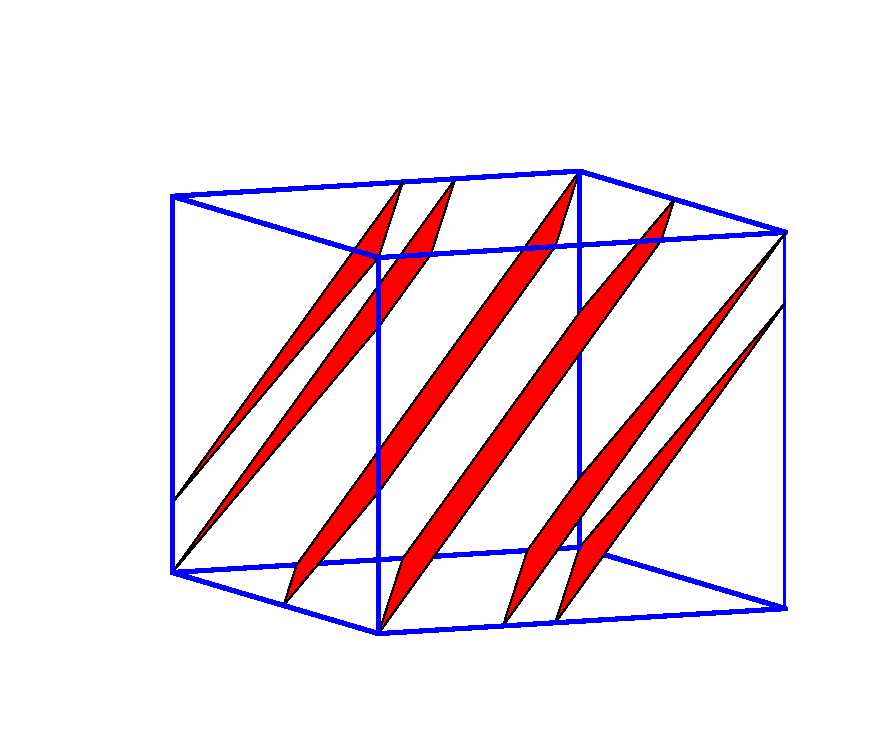
\includegraphics[width=0.4\textwidth]{multiplane.eps}
%\caption{fig1}
\label{fig:multiplane}
}
\quad
\subfigure[]{
\centering
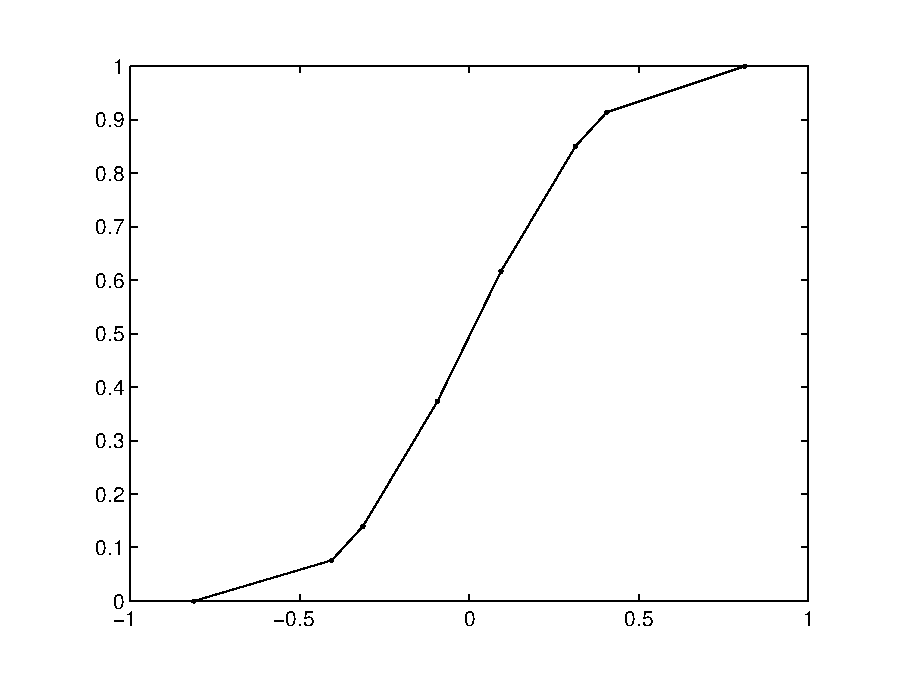
\includegraphics[width=0.4\textwidth]{piecewisefunction.eps}
\label{fig:piecewise}
%\caption{fig2}
}
%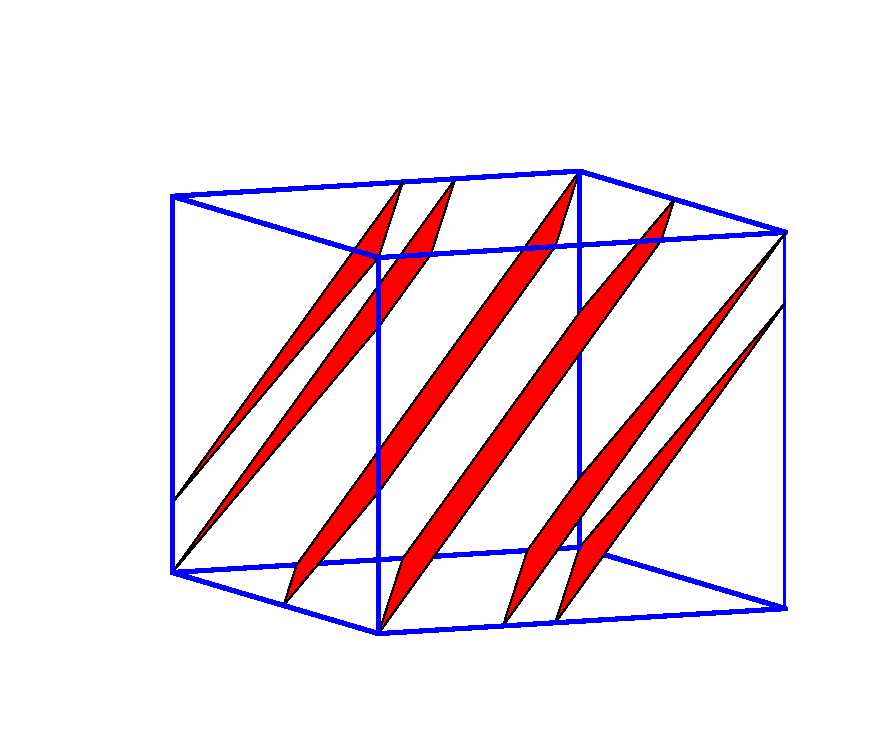
\includegraphics [width=0.5\textwidth]{multiplane.eps}
\caption{\subref{fig:multiplane} shows that planes pass different vertexes with the same normal direction. \subref{fig:piecewise} shows the cut volume and distance to the plane.}
\label{fig:multi}
\end{figure}

\subsection{Narrow band containing interface}
The cells that contain the interface are limited to where $H\in(\xi,1-\xi)$. $\xi$ is defined by users to confine the algorithm resolution, usually set as $0.0001$. The reason why uses Heaviside function rather than void fraction is that the interface defined by Heaviside function is more explicit and void fraction function more smeared. However, only interface cells are not enough to reconstruct the details of the interface. Level set method needs to build the signed distance function in the whole field, which can precisely capture the interface. Nonetheless, it takes too much computational resource and time to calculate on the whole field. So it is necessary to build a narrow band that has a thickness of two layers of grid like figure(\ref{fig:NarrowBand}). The first step is to sign all the interface cells with the flag "seed" and all the non-interface cell with the flag "away". The second step is to find the cells that share the vertexes of the "seed" cell. If the cells are signed with flags including "away" or "second layer", sign them with the flag "first layer". The third step is to traverse the cells that share the vertexes of the "first layer" cells. If the cells are signed with flags "away", sign them with the flag "second layer". Thus the narrow band that contains the interface and two-layers grids is built. The Heaviside function field and normal direction vector field can be limited in the narrow band to evade unnecessary computation.
\begin{figure}[htbp]
\centering
\includegraphics[width=0.5\textwidth]{band.eps}
\caption{The numbers in cells mean the flag. 0: "seed", 1:"first layer", 2:"second layer" and 4:"away"}
\label{fig:NarrowBand}
\end{figure}

\subsection{Reinitialization}

\subsection{Correction for mass conservation}

\subsection{Numerical Discretization of level set equation}


\section{Results}
In the following, some test cases with CLSAdvection method are presented. It is known that the level set method can improve the sharpness of the interface but also cause mass loss. Whereas, the volume of fluid method keeps the interface mass conservative but smeared. Therefore, the validation of the CLSAdvection method is tested in this article's work and there are several simple cases comparing this coupled method with the level set method and volume of fluid method. The error measures will be used to quantify the solution quality with following aspects.\\
--- Volume conservation\\
In order to track the precision of the advection process, volume conservation is measured to testify whether the simulated results conform to Navier-Stokes equations' requirement. The fractional volume conservative error is defined as following equation by this article\cite{gopala2008volume},
\begin{equation}\label{28}
\varepsilon_{V}(t)=\frac{\left|\sum\limits^N_{i=1}\alpha_i(t)V_i-\sum\limits^N_{i=1}\alpha_i(0)V_i\right|}{\sum\limits^N_{i=1}\alpha_{i}(0)V_i}.
\end{equation}
--- Mass conservation\\
The introduction of level set method that can cause the loss of mass for using equation (\ref{16}) to define the density may underlie a slight mass loss. Nevertheless, the coupled method is aimed to improve the algorithm's ability of mass conservation, which is measured by the following equation,
\begin{equation}\label{29}
\varepsilon_{M}(t)=\frac{\left|\sum\limits^N_{i=1}\rho_i(t)V_i-\sum\limits_{i=1}^N\rho_i(0)V_i\right|}{\sum\limits^N_{i=1}\rho_i(0)V_i}.
\end{equation}
--- Sharpness\\
The interface is shaper, the width of the region where $\alpha$ changes from 0 to 1 is thinner. Therefore, the following equation measures the sharpness.
\begin{equation}\label{30}
\varepsilon_{S}(t)=\frac{\sum_j\alpha_j(t)V_j}{\sum_i\alpha_i(t)V_i},
\end{equation}
where $j$ means the cells where $0.01\leq\alpha_j(t)\leq{0.99}$.\\
--- Boundedness\\
Volume fractions need to be physically meaningful, which means the condition $0\leq\alpha\leq{1}$ should be met. The measures of boundedness is $\min{(\alpha)}$ and $\max{(\alpha)}$. The measurements are taken all over the domain at the end of the calculation.\\ 
--- Efficiency\\
Efficiency is measured by the simulation times $T_{calc}$. All the simulation were executed on a single core of an Intel$^{\textregistered}$ 2.80 GHz CPU(i7-7700HQ) on a Dell$^{\textregistered}$ Precision 3520 Mobile Workstation.
We compare CLSAdvection's performance with an algebraic VOF scheme\citep{deshpande2012evaluating} and a geographic VOF scheme\citep{roenby2016computational} to benchmark the algorithm. Both the VOF schemes are implemented in the OpenFOAM$^{\textregistered}$ and well developed for arbitrarily unstructured meshes.
\subsection{Zalesak's test problem}
Solid body rotation of a notched disc is commonly used to test the advection capabilities of an interface capture solver. Zalesak firstly introduced this test \citep{zalesak1979fully} and its variants have been used extensively. In this particular test, the radius of the disc is $R=0.15$, the notch width is $W=0.06$ and the notch height is $H=0.25$. The center of the disc lies in $(x_0,y_0)=(0.5,0.75)$ in a domain of $1\times{1}$ that is discretized using rectangular meshes of size $100\times{100}$,$200\times{200}$,$400\times{400}$ figure (\ref{fig:hex0}). The rotation velocity is given by the following equation,
\begin{equation}\label{27}
\begin{split}
&u=-2\pi(y-0.5)
\\
&v=2\pi(x-0.5).
\end{split}
\end{equation}
At all the domain boundary, zero gradient condition is set for $\alpha$ and $\phi$. 

\subsubsection{structured meshes}
In figure (\ref{fig:MULESHEX},\ref{fig:ISOHEX},\ref{fig:CLSHEX}), the solutions of five combinations of time and mesh resolution in columns are obtained with MULES, isoAdvector, CLSAdvection. The effects of refining mesh resolution are investigated with fixed Courant Number, $Co=0.5$. With the finest mesh, the effects of reducing $Co$ from $0.5$ to $0.1$ are tested. Errors and Efficiency measures are displayed in table \ref{Tab:01}. Then we can get the following observations. All the algorithms are able to realize the volume conservation. But CLSAdvection method can cause slightly mass loss, which is confined at $0.01$. Especially, CLSAdvection can get the same sharpness as isoAdvector which is a sharp interface advection method and far better sharpness than the MULES method. Both isoAdvector and CLSAdvection method can make sure the void fraction $\alpha$ bounded at $[0,1]$. And MULES algorithm can cause a slight over flow. From table (\ref{Tab:01}), we can see the coupled VOF and level set method take the most time to finish the cases, which is caused by solving reinitialization equation (\ref{11}) and level set equation (\ref{10}). Besides, from table (\ref{Tab:01}), the influence of Courant number is that the smaller $Co$ means smaller time steps and the longer simulation time. Nevertheless, shrinking Courant number doesn't mean to improve the precision. Actually, the errors can be accumulated as the simulations process. From the figure (\ref{fig:CLSHEX}) and figure (\ref{fig:ISOHEX}), the shape of the notched disc is kept well at $Co=0.5$ and deforms more explicitly in the cases of $Co = 0.1$ and $Co = 0.2$. On the other hand, the results show that MULES method can cause numerical oscillations. As the meshes are densified, the oscillations become apparent, which can be explained by introducing high resolution convection scheme including vanLeer, SuperBee, QUICK and so on \cite{deshpande2012evaluating}.

\subsubsection{unstructured meshes}
We apply such algorithm on unstructured meshes and the initial shapes in figure (\ref{fig:poly0}) and figure (\ref{fig:trio0}). Figure (\ref{fig:MULESPoly}), (\ref{fig:ISOPoly}) and (\ref{fig:CLSPoly})show calculation results of MULES, isoAdvector, CLSAdvection after a circle in polygon meshes. And figure (\ref{fig:MULESTri}), (\ref{fig:ISOTri}) and (\ref{fig:CLSTri})show calculation results of MULES, isoAdvector, CLSAdvection after a circle in triangle meshes. The $Co$ numbers are set as $0.1$ and $0.5$, while the meshes have three different resolutions with the cell number 51967 and 203965. The errors and calculation times are showed in table \ref{Tab:02} and \ref{Tab:03}. From the figures and tables, we can make such conclusions as follows. First, the basic function of coupled level set and VOF method can be realized in unstructured meshes. The cell cut algorithm can be applied in polygon and triangle meshes. Second, the CLSAdvection can get the same sharpness effect as the sharp interface method, isoAdvector. MULES method can cause the interface smeared. After all, CLSAdvection inherits the idea of geometric volume of fluid method and explicitly reconstruct the interface. Third, polygon meshes are proved to have the better interface capturing capability than triangle meshes. Apparently, structured meshes undoubtedly have the best calculation characteristic. However, the nature of widely applied CFD softwares like OpenFOAM$^{\textregistered}$ and Fluent$^{\textregistered}$ requires the algorithm should be applied into unstructured meshes.

%\subsection{Spiraling Disc}
The deformation of a circle spiraling in a single vortex flow field is simulated to test the solver performance. The initial condition for the spiraling disc is like figure \ref{•}. The domain is the unit square with a disc of radius $R=0.15$ that is located at $(x,y) = (0.5,0.75)$. The Courant number is set as $Co = 0.5$. The velocity field is given by the following equation,
\begin{equation}
\label{31}
\mathbf{u}(x,y,t)=\cos{\frac{2\pi{t}}{T}}( -\sin^2(\pi{x})\sin(2\pi{y}),\sin(2\pi{x})\sin^2(\pi{y})),
\end{equation}
where the period of the flow is set to $T=16$. At time $T=4$, the disc is stretched into a long filament. At time $T=8$, the disc should recover to its initial shape. Therefore, the shape preservation error can be measured by comparing the computed final shape with the initial shape. Figure \ref{•} shows the shape preservation with MULES, isoAdvector and CLSAdvection methods in three different resolutions. And figure \ref{•} shows the spiraling disc in square, triangle and polygon meshes in three different resolutions on which the CLSAdvection method was tested and compared with other two methods, MULES and isoAdvector. Table \ref{} gives the error measures and calculation times at different mesh sizes and shapes.  

From the figure \ref{}, it is found that all simulations show some degree of pinching at $T=4$. The reason is that the filament thickness reaches the cell size. The coarsest mesh has the worst resolution and pinching is most pronounced. 
\subsection{Dam Break}
Here we test the CLSAdvection on the 2D dam break problem. This part we compare the CFD simulation results with the experiments made by Hu and Kashiwagi \cite{•} for validation. The water tank with a removable partition is showed in figure \ref{}. 
The figure \ref{} shows the simulation results using the MULES, isoAdvector and CLSADvection methods and the experiment pictures.
\subsection{Droplet}
Here we test the CLSAdvection on the 2D droplet distortion problem. This part we compare the CFD simulation results with the CFD results made by Hu and Kashiwagi \cite{•} for validation.
The figure \ref{} shows the simulation results using the MULES, isoAdvector and CLSADvection methods and the experiment pictures.

\section{Conclusions}

%%Vancouver style references.
\bibliographystyle{model1-num-names}
\bibliography{refs}

%\section*{Supplementary Material}

\end{document}

%%
